
\documentclass[12pt,a4paper]{article}
\usepackage{fullpage}
\usepackage[USenglish]{babel}
\usepackage{authblk}
\usepackage{hyperref}
\usepackage{graphicx}
\usepackage{listings}
\usepackage{xcolor}

\colorlet{punct}{red!60!black}
\definecolor{background}{HTML}{EEEEEE}
\definecolor{delim}{RGB}{20,105,176}
\colorlet{numb}{magenta!60!black}

\lstdefinelanguage{json}{
    basicstyle=\normalfont\ttfamily,
    numbers=left,
    numberstyle=\scriptsize,
    stepnumber=1,
    numbersep=8pt,
    showstringspaces=false,
    breaklines=true,
    frame=lines,
    backgroundcolor=\color{background},
    literate=
     *{0}{{{\color{numb}0}}}{1}
      {1}{{{\color{numb}1}}}{1}
      {2}{{{\color{numb}2}}}{1}
      {3}{{{\color{numb}3}}}{1}
      {4}{{{\color{numb}4}}}{1}
      {5}{{{\color{numb}5}}}{1}
      {6}{{{\color{numb}6}}}{1}
      {7}{{{\color{numb}7}}}{1}
      {8}{{{\color{numb}8}}}{1}
      {9}{{{\color{numb}9}}}{1}
      {:}{{{\color{punct}{:}}}}{1}
      {,}{{{\color{punct}{,}}}}{1}
      {\{}{{{\color{delim}{\{}}}}{1}
      {\}}{{{\color{delim}{\}}}}}{1}
      {[}{{{\color{delim}{[}}}}{1}
      {]}{{{\color{delim}{]}}}}{1},
}

\lstdefinelanguage{tableJson}{
    basicstyle=\small\ttfamily,
    showstringspaces=false,
    breaklines=true,
    aboveskip=0,
    belowskip=0,
    literate=
     *{0}{{{\color{numb}0}}}{1}
      {1}{{{\color{numb}1}}}{1}
      {2}{{{\color{numb}2}}}{1}
      {3}{{{\color{numb}3}}}{1}
      {4}{{{\color{numb}4}}}{1}
      {5}{{{\color{numb}5}}}{1}
      {6}{{{\color{numb}6}}}{1}
      {7}{{{\color{numb}7}}}{1}
      {8}{{{\color{numb}8}}}{1}
      {9}{{{\color{numb}9}}}{1}
      {:}{{{\color{punct}{:}}}}{1}
      {,}{{{\color{punct}{,}}}}{1}
      {\{}{{{\color{delim}{\{}}}}{1}
      {\}}{{{\color{delim}{\}}}}}{1}
      {[}{{{\color{delim}{[}}}}{1}
      {]}{{{\color{delim}{]}}}}{1},
}


\usepackage{todonotes}

% Remove section numbering
\setcounter{secnumdepth}{0}
% Remove paragraph indentation
\setlength{\parindent}{0cm}


\title{eBay Search Service \\[1ex] \large Preliminary Draft}
\author{Isabel Giang}
\author{Maxwell Wenger}
\affil{CSS490 Group Y4}

\date{January 26, 2021}


\begin{document}
\maketitle
\setcounter{tocdepth}{3}
\tableofcontents

% Problem:
% EBay Search has gotten quite slow.  We were able to gain some time by adding
% an index to the Master DB, but we are worried about long term scaling.  We
% need to settle on a design for a SearchServce that would be used to search
% for Auctions by Keyword and/or Category (breadcrumb)

% Deliverables:
% Create a design document that explains how you would solve the search
% problem.  This document will be read by the various engineers in the company
% for evaluation of your approach,so your design needs to be understandable to
% them based on the document.

\pagebreak
\section{Overview}
\subsection{Problem Statement}
In the last few months, eBay users have reported increasingly slow response
times from eBay's website when searching for auctions. Application log analysis
for the eBay Master Service has confirmed that our FindAuctions API for the
eBay Master service takes significantly longer to return a response when we
search for auctions using keywords. It also takes longer to search for a large
number of auctions.
\vspace{\baselineskip}
This is negatively impacting eBay's user experience for existing users and is
hindering the website's chances of being adopted by new users.

% State business problem
\vspace{\baselineskip}

Performing further analysis on the eBay Master service schema shows that the
FindAuctions API must scan the entire table to first find active auctions. Then
it must scan those active auctions to find auctions that have titles with the
keywords we are looking for.

\subsection{Temporary Solution}

As a bandaid solution to temporarily address this problem, we have added an 
AuctionStatus index to the Auction table of the eBay Master Service database.
This allows us to immediately access all active auctions instead of being forced 
to scan the entire Auction table to find active auctions before querying with keywords. 

\vspace{\baselineskip}
This speeds up the FindAuctions API enough to fix the poor user experience
temporarily, but this will not be enough as the company grows. The number of
records in the Auction table, and subsequently, the number of active auctions
will increase at an exponential rate.

\subsection{Next Steps}
To solve this more permanently, we want to create a separate search service
that will handle searching for auctions by keyword and/or category. 
We will call this new service the eBay Search Service.

\vspace{\baselineskip}
This search service will have its own database that can only be changed
by external users via its API. Whenever a new FindAuction API request is made, 
this service will perform the required business logic and databases accesses 
instead of the eBay Master service.

The eBay Search Service  will support searching in the following ways:

\begin{itemize}
\item Searching for all auctions
\item Searching for auctions based on auction status (closed, open, pending, cancelled)
\item Searching for auctions based on keywords
\item Searching for auctions based on category
\item Searching for auctions based on keywords and category
\end{itemize}

\pagebreak
% Clarify what kinds of searching we are doing such as:
% - Allow searching for only active auctions 
% - this one -> Allow searching for any auction.
% - Allow a bidder to find all of their active auctions
% - Administrator looking for a specific set of auctions that have expired
% - Etc

% Need Database Schema
 
\section{eBay Search Service API Specification}

\subsection{API List}
\begin{center}
    \begin{tabular}{| l | l |}
        \hline
        \textbf{API Name} & \textbf{Description} \\
        \hline
            createSearchableAuction & Creates an auction. \\ 
        \hline
            updateSearchableAuction & Updates an auction. \\
        \hline
            findAuctions & Finds auctions based on the given keywords and/or category. \\
        \hline
    \end{tabular}
\end{center}

\subsection{Schemas}

\subsubsection{SearchDB}
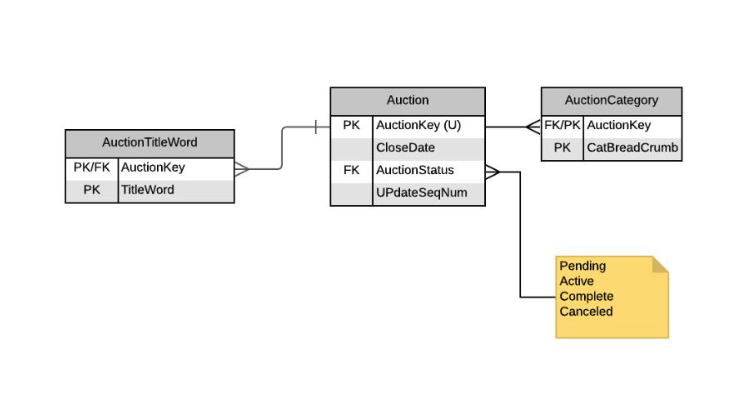
\includegraphics[scale=0.5]{images/Screen Shot 2021-01-22 at 11.34.49 PM.png}

\subsubsection{MasterDB}
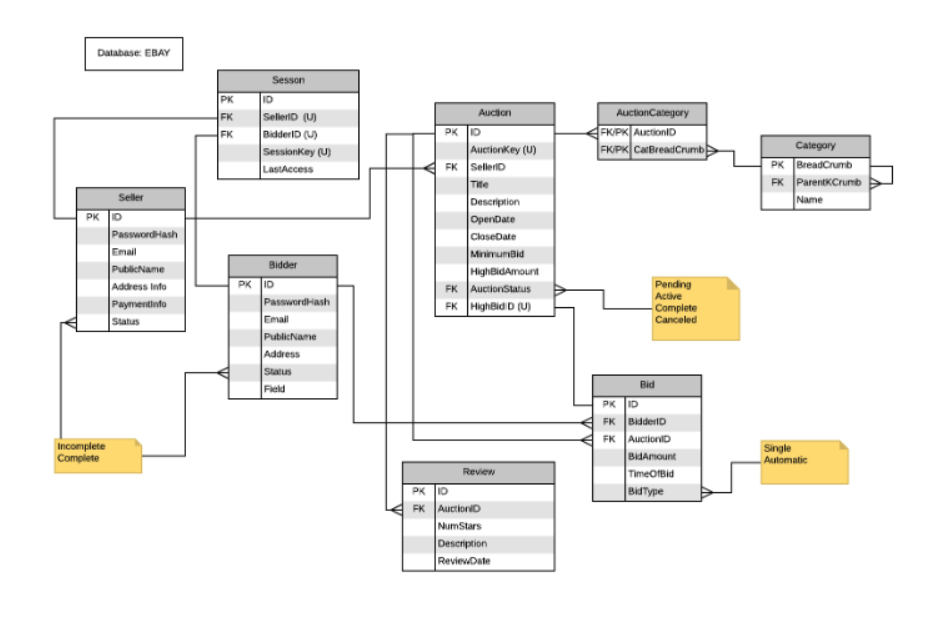
\includegraphics[scale=0.5]{images/Screen Shot 2021-01-24 at 9.45.28 PM.png}
\pagebreak
\subsection{API Descriptions}

\subsubsection{createSearchableAuction}
\label{ref:csa}
Creates an auction that is searchable by keywords and category. 


\paragraph{Input}

\begin{itemize}
    \item \textbf{auctionKey} - Public key that uniquely identifies an auction from the eBay Master Service.
    \item \textbf{title} - Title of the auction 
    \item \textbf{closeDate} - Closing date of the auction (ISO-8601 timestamp)
    \item \textbf{category} - Category breadcrumb
    \item \textbf{status} - Status of the auction (closed, open, pending, cancelled)
\end{itemize}
\begin{lstlisting}[language=json,numbers=none]
{
    "auctionKey": <string>,
    "title": <string>,
    "closeDate": <string>,
    "category": <string>,
    "status": <string>
}
\end{lstlisting}

\paragraph{Output}
\begin{center}
    \begin{tabular}{| p{7cm} | l |}
        \hline
        \textbf{Scenario} & \textbf{Response} \\
        \hline
        Successfully created an auction & 
        \begin{lstlisting}[language=tableJson,firstnumber=1]
{
    "success": true,
}

        \end{lstlisting} \\ 
        
        % \hline
         %    TODO: Make error states & Yeah! What he said! \\
        \hline
    \end{tabular}
\end{center}

\pagebreak
\subsubsection{updateSearchableAuction}
\label{ref:usa}
Updates the auction that corresponds with the given auction key.


\paragraph{Input}

\begin{itemize}
    \item \textbf{auctionKey} - Key that uniquely identifies the auction
    \item \textbf{title} - Title of the auction 
    \item \textbf{closeDate} - Closing date of the auction (ISO-8601 timestamp)
    \item \textbf{status} - Status of the auction (closed, open, pending, cancelled)
    \item \textbf{category} - Category breadcrumb
\end{itemize}
\begin{lstlisting}[language=json,numbers=none]
{
    "auction_key": <string>,
    "title": <string>, // optional
    "closeDate": <string>, // optional
    "status": <string>, // optional
    "category": <string> // optional
}
\end{lstlisting}

\paragraph{Output}
\begin{center}
    \begin{tabular}{| p{7cm} | l |}
        \hline
        \textbf{Scenario} & \textbf{Response} \\
        \hline
        Successfully updated an auction &
        \begin{lstlisting}[language=tablejson,firstnumber=1]
{
    "success": true
}
        \end{lstlisting} \\ 
        \hline
        The given auction key does not correspond to an auction. & 
        \begin{lstlisting}[language=tablejson,firstnumber=1]
{
    "success": false,
    "exception": "auctionkeynotfound"
}
        \end{lstlisting} \\
       %  \hline
       %      todo: make error states & yeah! what he said! \\
        \hline
    \end{tabular}
\end{center}

\pagebreak
\subsubsection{findAuctions}
Finds biddable auctions based on the given category and/or keywords. 

Entries will be ordered from
oldest to newest, starting from the pageIndex if given. 

If no pageIndex is
provided, findAuctions will return numResults number of results starting from
the first result.

\paragraph{Input} 

\begin{itemize}
    \item \textbf{keywords} - Keywords that auction results will be matched to
    \item \textbf{category} - Category breadcrumb
    \item \textbf{status} - Status of the auction (closed, open, pending, cancelled)
    \item \textbf{pageIndex} - Index where pagination begins. If given, results will be returned starting from this page.
    \item \textbf{numResults} - Number of auctions returned per page
\end{itemize}

\begin{lstlisting}[language=json,numbers=none]
{
    "keywords": [ <string>, ...], // optional
    "status": <string>, // optional
    "category": <string>, // optional
    "pageIndex": <number>, // optional
    "numResults": <number>
}
\end{lstlisting}

\paragraph{Output}
\begin{center}
    \begin{tabular}{| p{7cm} | l |}
        \hline
        \textbf{scenario} & \textbf{response} \\
        \hline
        Successfully search with found results. &
        \begin{lstlisting}[language=tablejson,firstnumber=1]
{
    "success": true,
    "results": [ 
        auctionKey: <string>,
        ...
    ],
    "pageIndex": <int>
}
        \end{lstlisting} \\ 
        \hline
 \hline
        Successfully search with no results. &
        \begin{lstlisting}[language=tablejson,firstnumber=1]
{
    "success": true,
    "results": [ ]
}
         \end{lstlisting} \\ 
        % \hline
         %    todo: make error states & yeah! what he said! \\
         \hline
    \end{tabular}
\end{center}

\pagebreak
\section{eBay Search Service Internals}
% Describe what internal processes you do based on APIs.
% I.E. What happens to DB when xyz is called.
\subsection{createAuction}
This creates an entry in the AuctionSearch database for the auction, all of the
auction's keywords, and the auction category.

\subsection{updateAuction}
Update searchable auction will update fields, keywords, and categories of an
existing auction in the search table.

New keywords will be generated if a new title is provided. The new keywords will be added to the database, and keywords
associated with they auction key but were not again generated from the updated
title will be removed from the database. The fields will be based on the
auction key, therefore the auction key may not be updated. Any optional fields
not included in the message to the service will not be changed.

\subsection{findAuctions}
The parameters search by ``anding'' the results together (e.g. if you ask for a
keyword ``red'', ``LG'' with the category ``ELE:PHO'' signifying phones in
electronics, red LG phones will be returned, but not red Nokia phones, or red
LG refrigerators). To perform searches that ``or'' search terms, multiple
searches must be made.

\pagebreak
\section{Changes to eBay Master Service}

\subsection{createAuction}

Creates an auction as it did before, although now the createAuction service is
responsible for calling createSearchableAuction to create a search entry for
the auction.

The impact on the database from createAuction is documented in the master api
documentation. The impact on the database from createSearchableAuction is
documented in section \nameref{ref:csa}.

If three calls to the search service fails, the call will be queued up to be
attempted again with other failed calls at a regular interval.

% For any changes to the ebay master service, we need to provide:
% - Description of schema changes (not a full schema drawing)
% - Description of behavioral changes
%   - Describe new control  flow
%   - Describe transactional events
%   - Describe what happens on timeout from the search service.
% - Any additional API calls that are needed to be added to master service

\subsection{updateAuction}

Update auction will work as it did before. Except, now, update auction will
call updateSearchableAuction with the updated parameters it will receive.

The impact on the database from updateAuction is documented in the master api
documentation. The impact on the database from updateSearchableAuction is
documented in section \nameref{ref:usa}.

If three calls to the search service fails, the call will be queued up to be
attempted again with other failed calls at a regular interval.

\pagebreak
\section{Logging}

This section describes a suggested format for this service's application logs.

\begin{lstlisting}[boxpos=t,language=json,firstnumber=1]
{
    "start": <string>,
    "duration": <string>,
    "api": <string>,
    "params":
        {
            "original": {
                "auctionkey": <string>,
                "title": <string>, // optional
                "closeDate": <string>, // optional
                "status": <string>, // optional
                "category": <string> // optional 
            }, 
            "updated": {
                "auctionkey": <string>,
                "title": <string>, // optional
                "closeDate": <string>, // optional
                "status": <string>, // optional
                "category": <string> // optional 
            }
        }
}           
\end{lstlisting}

\begin{itemize}
    \item \textbf{start} The time the service first receives the call.
    \item \textbf{duration} The amount of time it takes from when the service
        receives the call to when the service responds.
    \item \textbf{api} The name of the API that is called.
    \item \textbf{params} The original and updated data that the API changed.
        Optional data that was not changed is not included in either the
        updated or original logs.
\end{itemize}


\end{document}
